%% abtex2-modelo-trabalho-academico.tex, v-1.7.1 laurocesar
%% Copyright 2012-2013 by abnTeX2 group at http://abntex2.googlecode.com/
%%
%% This work may be distributed and/or modified under the
%% conditions of the LaTeX Project Public License, either version 1.3
%% of this license or (at your option) any later version.
%% The latest version of this license is in
%%   http://www.latex-project.org/lppl.txt
%% and version 1.3 or later is part of all distributions of LaTeX
%% version 2005/12/01 or later.
%%
%% This work has the LPPL maintenance status `maintained'.
%%
%% The Current Maintainer of this work is the abnTeX2 team, led
%% by Lauro C\'{e}sar Araujo. Further information are available on
%% http://abntex2.googlecode.com/
%%
%% This work consists of the files abntex2-modelo-trabalho-academico.tex,
%% abntex2-modelo-include-comandos and abntex2-modelo-references.bib
%%

% ------------------------------------------------------------------------
% ------------------------------------------------------------------------
% abnTeX2: Modelo de Trabalho Academico (tese de doutorado, dissertacao de
% mestrado e trabalhos monograficos em geral) em conformidade com
% ABNT NBR 14724:2011: Informacao e documentacao - Trabalhos academicos -
% Apresentacao
% ------------------------------------------------------------------------
% ------------------------------------------------------------------------

%ARQUIVO DE PREAMBULO DA TESE - PACOTES E CONFIGURA\c{C}\~{O}ES

\documentclass[
	% -- op\c{c}\~{o}es da classe memoir --
	12pt,				% tamanho da fonte
	openright,			% cap\'{\i}tulos come\c{c}am em p\'{a}g \'{\i}mpar (insere p\'{a}gina vazia caso preciso)
	oneside,			% para impress\~{a}o em verso e anverso. Oposto a oneside
	a4paper,			% tamanho do papel.
	% -- op\c{c}\~{o}es da classe abntex2 --
	%chapter=TITLE,		% t\'{\i}tulos de cap\'{\i}tulos convertidos em letras mai\'{u}sculas
	%section=TITLE,		% t\'{\i}tulos de se\c{c}\~{o}es convertidos em letras mai\'{u}sculas
	%subsection=TITLE,	% t\'{\i}tulos de subse\c{c}\~{o}es convertidos em letras mai\'{u}sculas
	%subsubsection=TITLE,% t\'{\i}tulos de subsubse\c{c}\~{o}es convertidos em letras mai\'{u}sculas
	% -- op\c{c}\~{o}es do pacote babel --
	english,			% idioma adicional para hifeniza\c{c}\~{a}o
	%french,			% idioma adicional para hifeniza\c{c}\~{a}o
	%spanish,			% idioma adicional para hifeniza\c{c}\~{a}o
	brazil,				% o \'{u}ltimo idioma \'{e} o principal do documento
	sumario=tradicional,
	]{abntex2}


% ---
% PACOTES
% ---

% ---
% Pacotes fundamentais
% ---
\usepackage{cmap}				% Mapear caracteres especiais no PDF
\usepackage{lmodern}			% Usa a fonte Latin Modern			
\usepackage[T1]{fontenc}		% Selecao de codigos de fonte.
\usepackage[utf8]{inputenc}		% Codificacao do documento (convers\~{a}o autom\'{a}tica dos acentos)
\usepackage{lastpage}			% Usado pela Ficha catalogr\'{a}fica
\usepackage{indentfirst}		% Indenta o primeiro par\'{a}grafo de cada se\c{c}\~{a}o.
\usepackage{color}				% Controle das cores
\usepackage[pdftex]{graphicx}	% Inclus\~{a}o de gr\'{a}ficos
\usepackage{epstopdf}           % Pacote que converte as figuras em eps para pdf
\usepackage{lipsum}             % Pacote que gera texto dummy
\usepackage{blindtext}          % Pacote que gera texto dummy
% ---
		
% ---
% Pacotes adicionais, usados apenas no \^{a}mbito do Modelo Can\^{o}nico do abnteX2
% ---
\usepackage{nomencl}
\usepackage{amsmath}
\usepackage{bbm}
\usepackage[chapter]{algorithm}
\usepackage{algorithmic}
\usepackage{multirow}
\usepackage{rotating}
\usepackage{pdfpages}
% ---

% ---
% Pacotes de cita\c{c}\~{o}es
% ---
\usepackage[brazilian,hyperpageref]{backref}	 % Paginas com as cita\c{c}\~{o}es na bibl
\usepackage[alf,abnt-etal-cite=2,abnt-etal-list=0,abnt-etal-text=emph]{abntex2cite}	% Cita\c{c}\~{o}es padr\~{a}o ABNT

% ---
% Pacote de customiza\c{c}\~{a}o - Unicamp
% ---
\usepackage{unicamp}


% ---
% CONFIGURA\c{C}\~{O}ES DE PACOTES
% ---

% ---
% Configura\c{c}\~{o}es do pacote backref
% Usado sem a op\c{c}\~{a}o hyperpageref de backref
\graphicspath{{./eps/}}
\DeclareGraphicsExtensions{.eps}

%customiza\c{c}\~{a}o do negrito em ambientes matem\'{a}ticos
\newcommand{\mb}[1]{\mathbf{#1}}
%customiza\c{c}\~{a}o de teoremas
\newtheorem{mydef}{Defini\c{c}\~{a}o}[chapter]
\newtheorem{lemm}{Lema}[chapter]
\newtheorem{theorem}{Teorema}[chapter]
\floatname{algorithm}{Pseudoc\'{o}digo}
\renewcommand{\listalgorithmname}{Lista de Pseudoc\'{o}digos}


\renewcommand{\backrefpagesname}{Citado na(s) p\'{a}gina(s):~}
% Texto padr\~{a}o antes do n\'{u}mero das p\'{a}ginas
\renewcommand{\backref}{}
% Define os textos da cita\c{c}\~{a}o
\renewcommand*{\backrefalt}[4]{
	\ifcase #1 %
		Nenhuma cita\c{c}\~{a}o no texto.%
	\or
		Citado na p\'{a}gina #2.%
	\else
		Citado #1 vezes nas p\'{a}ginas #2.%
	\fi}%
% ---


% ---
% Configura\c{c}\~{o}es de apar\^{e}ncia do PDF final

% alterando o aspecto da cor azul
\definecolor{blue}{RGB}{41,5,195}

% informa\c{c}\~{o}es do PDF
\makeatletter
\hypersetup{
     	%pagebackref=true,
		pdftitle={\@title},
		pdfauthor={\@author},
    	pdfsubject={\imprimirpreambulo},
	    pdfcreator={LaTeX with abnTeX2},
		pdfkeywords={abnt}{latex}{abntex}{abntex2}{trabalho acad\^{e}mico},
		hidelinks,					% desabilita as bordas dos links
		colorlinks=false,       	% false: boxed links; true: colored links
    	linkcolor=blue,          	% color of internal links
    	citecolor=blue,        		% color of links to bibliography
    	filecolor=magenta,      	% color of file links
		urlcolor=blue,
%		linkbordercolor={1 1 1},	% set to white
		bookmarksdepth=4
}
\makeatother
% ---

% ---
% Espa\c{c}amentos entre linhas e par\'{a}grafos
% ---

% O tamanho do par\'{a}grafo \'{e} dado por:
\setlength{\parindent}{2cm}

% Controle do espa\c{c}amento entre um par\'{a}grafo e outro:
\setlength{\parskip}{0.2cm}  % tente tamb\'{e}m \onelineskip

% ---
% Informacoes de dados para CAPA e FOLHA DE ROSTO
% ---
\titulo{T\'{\i}tulo da Disserta\c{c}\~{a}o/Tese}
\autor{Nome do Autor}
\local{Campinas}
\data{Ano da defesa}
\orientador{Prof. Dr. Orientador}
\coorientador[Co-orientador]{Prof. Dr. Co-orientador}
\instituicao{%
    UNIVERSIDADE ESTADUAL DE CAMPINAS
    \par
    Faculdade de Engenharia El\'{e}trica e de Computa\c{c}\~{a}o	
    }
%\tipotrabalho{Tese (Doutorado)}
%% O preambulo deve conter o tipo do trabalho, o objetivo, o nome da institui\c{c}\~{a}o e a \'{a}rea de concentra\c{c}\~{a}o
%\preambulo{Tese apresentada \`{a} Faculdade de Engenharia El\'{e}trica e de Computa\c{c}\~{a}o da Universidade Estadual de Campinas como parte dos requisitos exigidos para a obten\c{c}\~{a}o do t\'{\i}tulo de Doutor em Engenharia El\'{e}trica, na \'{A}rea de Engenharia de Computa\c{c}\~{a}o.}
\tipotrabalho{Disserta\c{c}\~{a}o (Mestrado)}
\preambulo{Disserta\c{c}\~{a}o apresentada \`{a} Faculdade de Engenharia El\'{e}trica e de Computa\c{c}\~{a}o da Universidade Estadual de Campinas como parte dos requisitos exigidos para a obten\c{c}\~{a}o do t\'{\i}tulo de Mestre em Engenharia El\'{e}trica, na \'{A}rea de xxx.}
% --- 

% ---- compila o \'{\i}ndice  ----
\makeindex
\makenomenclature
% ---

% ---- In\'{\i}cio do documento ----
\begin{document}

% Retira espa\c{c}o extra obsoleto entre as frases.
\frenchspacing

% ---- ELEMENTOS PR\'{E}-TEXTUAIS ----
\pretextual

% --- Capa ---
\imprimircapa
% ---

% --- Folha de rosto (o * indica que haver\'{a} a ficha catalogr\'{a}fica) ---
\setcounter{page}{2}
\imprimirfolhaderosto*
% ---

% --- Inserir a ficha catalogr\'{a}fica ---

% Isto \'{e} um exemplo de Ficha Catalogr\'{a}fica, ou ``Dados internacionais de
% cataloga\c{c}\~{a}o-na-publica\c{c}\~{a}o''. Voc\^{e} pode utilizar este modelo como refer\^{e}ncia.
% Por\'{e}m, provavelmente a biblioteca da sua universidade lhe fornecer\'{a} um PDF
% com a ficha catalogr\'{a}fica definitiva ap\'{o}s a defesa do trabalho. Quando estiver
% com o documento, salve-o como PDF no diret\'{o}rio do seu projeto e substitua todo
% o conte\'{u}do de implementa\c{c}\~{a}o deste arquivo pelo comando abaixo:

% --- Para a vers\~{a}o final, delete as linhas abaixo e insira a linha do \includepdf
 \begin{fichacatalografica}
    \vspace*{\fill}
    \begin{center}
        \textsc{Inclua aqui o pdf com a ficha catalogr\'{a}fica fornecida pela BAE.}
    \end{center}
    \vspace*{\fill}
% --- --- ---
    %\includepdf{ficha-catalografica.pdf}
 \end{fichacatalografica}
% ---


% --- Inserir folha de aprova\c{c}\~{a}o ---

% Isto \'{e} um exemplo de Folha de aprova\c{c}\~{a}o, elemento obrigat\'{o}rio da NBR
% 14724/2011 (se\c{c}\~{a}o 4.2.1.3). Voc\^{e} pode utilizar este modelo at\'{e} a aprova\c{c}\~{a}o
% do trabalho. Ap\'{o}s isso, substitua todo o conte\'{u}do deste arquivo por uma
% imagem da p\'{a}gina assinada pela banca com o comando abaixo:

\newpage
\begin{center}
\textbf{\textsc{Comissão Julgadora -- Dissertação de Mestrado}}\\[1cm]
\end{center}

\noindent\textbf{Candidato:} [INSERIR NOME] \quad RA [INSERIR RA] \\
\noindent\textbf{Data de defesa:} [DIA] de [MES] de [ANO] \\

\noindent\textbf{Título da dissertação:} \noindent ``\thetitle'' \\[2cm]
Prof. Dr. [NOME ORIENTADOR] (Presidente, FEEC/UNICAMP) \\[1pt]
Prof. Dr. [NOME MEMBRO EXTERNO] ([FILIACAO MEMBRO EXTERNO)\\[1pt]
Prof. Dr. [NOME MEMBRO INTERNO] ([FILIACAO MEMBRO INTERNO)\\[2cm]
\noindent
A ata de defesa, com as respectivas assinaturas dos membros da Comissão Julgadora, encontra-se no processo de vida acadêmica do aluno.\\

\vspace*{\fill}
\newpage
% --- --- ---
%\includepdf[pagecommand={\thispagestyle{plain}}]{folha-assinaturas.pdf}   
\cleardoublepage

% ---


% --- Dedicat\'{o}ria ---
\begin{dedicatoria}
    \vspace*{\fill}
    \centering
    \noindent
    \textit{Dedico esta tese \`{a} todo mundo.}
    \vspace*{\fill}
\end{dedicatoria}
% ---

% --- Agradecimentos ---
\begin{agradecimentos}
    \lipsum[1-3]
\end{agradecimentos}
% ---

% --- Ep\'{\i}grafe  ---
\begin{epigrafe}
    \vspace*{\fill}
	\begin{flushright}
		\textit{``Escreva aqui a sua ep\'{\i}grafe''\\
		(Cita\c{c}\~{a}o)}
	\end{flushright}
\end{epigrafe}
% ---


% --- RESUMOS (em portugu\^{e}s e ingl\^{e}s ---

\begin{resumo}
    \lipsum[1]
    \vspace{\onelineskip}

    \noindent\textbf{Palavras-chaves}: palavra-chave 1; palavra-chave 2; palavra-chave 3.

    \vspace{\onelineskip}
    \vspace{\onelineskip}

    \begin{otherlanguage*}{english}
    \begin{center}{\ABNTEXchapterfont\huge Abstract}\end{center}
    \lipsum[2]

    \vspace{\onelineskip}

    \noindent\textbf{Keywords}: keyword 1; keyword 2; keyword 3.

    \end{otherlanguage*}
\end{resumo}
% ---

% --- inserir lista de ilustra\c{c}\~{o}es ---
\pdfbookmark[0]{\listfigurename}{lof}
\listoffigures*
\cleardoublepage
% ---

% --- inserir lista de tabelas ---
\pdfbookmark[0]{\listtablename}{lot}
\listoftables*
\cleardoublepage
% ---

% --- inserir lista de Acronimos e Abrevia\c{c}\~{o}es ---
\renewcommand{\nomname}{Lista de Acr\^{o}nimos e Abrevia\c{c}\~{o}es}
\pdfbookmark[0]{\nomname}{las}
\printnomenclature
\cleardoublepage
% ---

% --- inserir o sumario ---
\pdfbookmark[0]{\contentsname}{toc}
\tableofcontents*
\cleardoublepage
% ---

% ---- ELEMENTOS TEXTUAIS ----
\textual

% ---- Introdu\c{c}\~{a}o ----

\chapter{Introdu\c{c}\~{a}o}
\label{cap:intro}
\lipsum[1-4]    % Dummy text para a introdu\c{c}\~{a}o

% ---- Cap\'{\i}tulos ----

\part{Fundamentos (Opcional)}

\chapter{Exemplo de T\'{\i}tulo}
\label{cap:cap01}

Lorem ipsum dolor sit amet, consectetur adipiscing elit. Vivamus tempus at lectus sed facilisis. Proin posuere id lacus in semper. Praesent semper justo non fringilla hendrerit. Mauris tempus in diam non lacinia. Integer ac lacus diam. Nullam et aliquet eros. In eget vestibulum neque. Mauris gravida erat eget augue sollicitudin laoreet. Suspendisse felis ipsum, sodales non sapien ut, pharetra posuere justo.

\section{Exemplo de Se\c{c}\~{a}o}
\label{sec:sec01}

Nunc malesuada posuere felis vel dapibus. Aliquam at fermentum lacus, vel malesuada elit. Duis varius nisi eget elit sagittis suscipit. Cras eu arcu at quam tristique facilisis eget vel ante. Quisque vitae libero lacinia, pellentesque tellus in, semper ligula. Aenean pharetra, elit vitae tristique pellentesque, justo erat luctus lectus, eget accumsan eros nisl vitae arcu. Proin consequat accumsan enim et porta. Aenean pharetra nulla risus, vitae ullamcorper ligula molestie in~\cite{Cover2006}.

Integer ut elit lacus. Nullam id ullamcorper metus, et tincidunt mi. Donec blandit, sapien sit amet ultricies pharetra, turpis elit mollis risus, et pulvinar risus magna sed nunc. Sed eget risus ac risus consequat congue et ac nunc. Aenean a eros magna. Sed vel ante id ante venenatis feugiat. Sed et tortor dictum, pulvinar erat et, tempus felis. Donec pretium sagittis augue, non lacinia felis luctus a.

\begin{equation}
H(X) =-K\sum_{x\in\mathcal{X}} p_X(x)\log p_X(x),
\label{eq:shannonEntropy1}
\end{equation}

A equa\c{c}\~{a}o pode ser citada assim~\eqref{eq:shannonEntropy1}, e a se\c{c}\~{a}o assim~\ref{sec:sec01}

Aenean mauris sem, vulputate vitae vulputate vel, imperdiet volutpat erat. Nam malesuada pellentesque orci ac blandit. Maecenas pulvinar augue ac metus porttitor, eget tristique nunc vulputate. Sed nec mi mi. Curabitur ultrices facilisis consectetur. Cras vel urna porttitor, porta quam a, facilisis libero. Cras volutpat diam in tempor iaculis. Quisque rutrum vestibulum elit, sit amet gravida quam elementum ac. Fusce pretium hendrerit libero sed luctus. Phasellus sodales tristique purus non bibendum. Aenean faucibus pulvinar ligula, ut aliquam eros varius adipiscing. Ut a ipsum tempor, placerat quam non, imperdiet mi.

\begin{figure}[htb]
\centering
	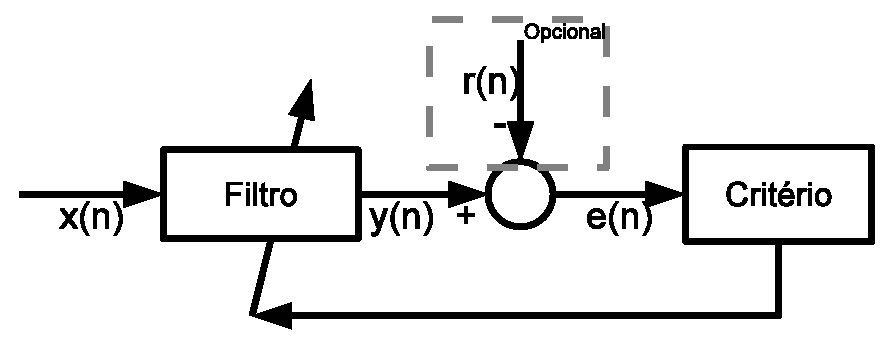
\includegraphics[width=.7\columnwidth]{cap1/filtering}
\caption{Esquema geral do problema de filtragem.}
\label{fig:filtering}
\end{figure}

Etiam id lobortis felis, dignissim commodo est. Nunc varius nulla et aliquam venenatis. Duis non neque ut tortor gravida viverra ut nec eros. Vestibulum et felis feugiat, lacinia ante et, tempus sem. Sed quis augue varius, sagittis lacus et, scelerisque felis. Morbi nec ligula ante. Maecenas vel sodales urna, vitae accumsan nisi. Maecenas lacinia adipiscing quam, eget elementum purus feugiat at. Fusce eget dictum sem. Maecenas ante ligula, tempus non mattis quis, ultrices vel elit. Nam porta est sit amet euismod pharetra. Integer vestibulum sem a sem volutpat, vitae adipiscing massa consequat. Aliquam iaculis mi in ultrices aliquet. Donec vitae semper sapien. Vivamus vel pretium enim.

Vestibulum ante ipsum primis in faucibus orci luctus et ultrices posuere cubilia Curae; Praesent porta ligula ipsum, ac lacinia leo malesuada ac. Morbi convallis in sapien at accumsan. Nunc sit amet tempus leo, adipiscing molestie leo. Sed ut arcu consequat lacus sagittis facilisis nec sit amet diam. Fusce a gravida dolor, eu sodales tellus. Ut porta nec velit at lacinia. Mauris felis arcu, faucibus eu porta vitae, luctus a nisl. Aenean tempus felis risus, sed vehicula ante fringilla quis. Integer eget purus a diam ultricies placerat. Donec consectetur vel urna id faucibus. In accumsan iaculis imperdiet. Nam venenatis enim quis nisl mattis, quis mattis neque tincidunt. Nullam sem enim, euismod ac nisi vel, viverra imperdiet augue.

\subsection{Subse\c{c}\~{a}o}
\label{sec:subsec01}

Maecenas condimentum nunc a tincidunt fermentum. Donec lobortis fermentum ante at hendrerit. Duis et gravida nisl. Nulla auctor dui sit amet mi tempor pretium eget fermentum nisi. Nam pharetra dolor eget ipsum consectetur porta. Ut ullamcorper enim a lacus dapibus, vel malesuada tellus posuere. Suspendisse sapien enim, cursus quis bibendum cursus, dapibus vel neque. Aliquam viverra, nulla in dictum dignissim, est nulla dapibus magna, id pretium tellus orci eget lacus. Interdum et malesuada fames ac ante ipsum primis in faucibus. Ut fermentum, erat at vulputate tempus, enim lorem elementum velit, eget tempus diam arcu at leo. Proin eu neque ac erat fermentum varius nec sit amet eros. Fusce arcu mi, consequat non nibh vel, tempus bibendum orci. Nulla vel nulla massa. Nullam sit amet velit aliquet, fringilla augue ac, congue nulla. Sed dignissim, magna eu posuere luctus, libero elit posuere sem, eu euismod ligula elit non sem.

Nullam lacinia ipsum vitae eros facilisis bibendum. Maecenas commodo neque dui, tristique porta sem ullamcorper ut. Vestibulum condimentum mauris eu egestas euismod. Nam vel ante congue libero accumsan mattis. Phasellus commodo euismod mi ac commodo. Proin quis volutpat massa. Curabitur non nunc sit amet augue placerat vulputate et fermentum arcu. In pellentesque lacinia tortor, quis vehicula arcu. Morbi lacinia vel ante ac tincidunt. Curabitur ac tincidunt eros.

Fusce id tellus nulla. Suspendisse aliquet sapien lacus, sit amet fermentum lacus pharetra a. Integer eu urna ut sem ultricies luctus in lacinia justo. Sed vel mattis orci, id egestas libero. Fusce ac libero aliquam neque faucibus cursus. Pellentesque pulvinar at nisl eget fermentum. Pellentesque quis interdum neque. Aenean vehicula euismod rutrum. Nulla luctus justo sit amet justo dignissim fermentum. Nunc eget ultrices dui, quis venenatis neque. Nullam volutpat nibh metus, sit amet convallis augue lacinia non. Maecenas eu est in nulla eleifend porttitor vel rutrum nisl.

Vestibulum erat purus, ultricies vehicula enim et, commodo posuere arcu. Pellentesque at orci metus. Aenean vestibulum mauris at nibh gravida, venenatis tempus augue sollicitudin. Curabitur nec justo odio. Cum sociis natoque penatibus et magnis dis parturient montes, nascetur ridiculus mus. Suspendisse varius ipsum at justo viverra mollis eu ac mauris. Nunc in facilisis erat. Ut aliquet tempus neque ac pretium. In viverra, risus imperdiet commodo commodo, orci tortor venenatis justo, sed ultricies nisi tortor at velit. Vivamus ultricies enim sit amet eleifend malesuada. Nullam at velit sem. Vivamus viverra tortor sed urna auctor interdum. 

\part{Contribui\c{c}\~{o}es (Opcional)}

\include{cap5}

% --- Finaliza a parte no bookmark do PDF, para que se inicie o bookmark na raiz ---
\bookmarksetup{startatroot}%
% ---

% --- Conclus\~{a}o ---
\chapter*[Conclus\~{a}o]{Conclus\~{a}o}
\addcontentsline{toc}{chapter}{Conclus\~{a}o}
\lipsum[1-5]

% ---- ELEMENTOS P\'{O}S-TEXTUAIS ----
\postextual

% ---- Refer\^{e}ncias bibliogr\'{a}ficas ----
\bibliography{tese}

% ---- Ap\^{e}ndices ----

% ---
% Inicia os ap\^{e}ndices
% ---
%\begin{apendicesenv}
%
%% Imprime uma p\'{a}gina indicando o in\'{\i}cio dos ap\^{e}ndices
%\partapendices
%
%% ----------------------------------------------------------
%\chapter{Quisque libero justo}
%% ----------------------------------------------------------
%
%\lipsum[50]
%
%% ----------------------------------------------------------
%\chapter{Nullam elementum urna vel imperdiet sodales elit ipsum pharetra ligula
%ac pretium ante justo a nulla curabitur tristique arcu eu metus}
%% ----------------------------------------------------------
%\lipsum[55-57]
%
%\end{apendicesenv}
% ---

% ---- Anexos ----

% ---
% Inicia os anexos - opcional
% ---
\begin{anexosenv}

% Imprime uma p\'{a}gina indicando o in\'{\i}cio dos anexos
\partanexos

% ---
\chapter{Morbi ultrices rutrum lorem.}
% ---
\lipsum[30]

% ---
\chapter{Cras non urna sed feugiat cum sociis natoque penatibus et magnis dis
parturient montes nascetur ridiculus mus}
% ---

\lipsum[31]

% ---
\chapter{Fusce facilisis lacinia dui}
% ---

\lipsum[32]

\end{anexosenv}

% ---- INDICE REMISSIVO ----

\printindex

\end{document} 